

% [doc] -----------------------------
% [doc] Instructions
% [doc] -----------------------------
% [doc] https://intranet.inria.fr/Vie-scientifique/Information-edition-scientifiques/RADAR/Structure-du-rapport
% [doc] -----------------------------

%% [BEGIN last year imported content]






% [radar] -----------------------------------
% [radar] Do not alter this section title
\section{Research program}
\label{diverse:research}
% [radar] -----------------------------------

\subsection{Context}

Applications are becoming more complex and the demand for faster development is increasing. In order to better adapt to the unbridled evolution of requirements in markets where software plays an essential role, companies are changing the way they design, develop, secure and deploy applications, by relying on:

\begin{itemize}
	\item A massive use of reusable libraries from a rich but fragmented eco-system;
	\item An increasing configurability of most of the produced software; 
	\item  A strongly increase in evolution frequency;
	\item Cloud-native architectures based on containers, naturally leading to a diversity of programming  languages used, and to the emergence of infrastructure, dependency, project and deployment descriptors (models); 
\item Implementations of fully automated software supply chains; 	
\item  The use of lowcode/nocode platforms;
\item The use of ever richer integrated development environments (IDEs),  more and more deployed in SaaS mode; 
\item The massive use of data and artificial intelligence techniques in software production chains.
\end{itemize}

\bigskip\noindent These trends are set to continue, all the while with a strong concern about the security properties of the produced and distributed software. 


\noindent The numbers in the examples below help to understand why this evolution of modern software engineering brings a \textbf{change of dimension}:
\begin{itemize}
	\item When designing a simple kitchen sink (\textit{hello world}) with the {\tt angular} framework, more than 1600 dependencies of JavaScript libraries are pulled. 
	\item  The numbers revealed by Google in~2018 showed that over 500~million tests are run \emph{per day} inside Google’s systems, leading to over 4 millions daily builds.
	\item Also at Google, they reported 86~TB of data, including two billion lines of code in nine million source files \footcite{potvin2016google}. Their software also rapidly evolves both in terms of frequency and in terms of size. Again, at Google, 25,000 developers typically commit 16,000 changes to the codebase on a single workday. This is also the case for most of software code, including open source software. 
	\item  x264, a highly popular and configurable video encoder, provides 100+ options that can take boolean, integer or string values. 
	There are different ways of compiling x264, and it is well-known that the compiler options (e.g., -O1 –O2 –O3 of gcc) can influence the performance of a software; the widely used gcc compiler, for example, offers more than 200~options. 
	The x264 encoder can be executed on different configurations of the Linux operating system, whose options may in turn influence x264 execution time; in recent versions ($>$ 5), there are 16000+ options to the Linux kernel.
	Last but not least, x264 should be able to encode many different videos, in different formats and with different visual properties, implying a
  huge variability of the input space. 
	Overall, the variability space is enormous, and ideally x264 should be run and tested in all these settings. 
	But a rough estimation shows that the number of possible configurations, resulting from the combination of the different variability layers, is~$10^{6000}$. 
    \end{itemize}


The \team{} research project is working and evolving in the context of this acceleration. 
We are active at all stages of the \textbf{software supply chain}.  
Software supply chain covers all the activities and all the stakeholders that relate to software production and delivery.
All these activities and stakeholders have to be smartly managed together as part of an overall strategy.
The goal of supply chain management (SCM) is to meet customer demands with the most efficient use of resources possible. 
 
In this context, \team{} is particularly interested in the following research questions: 
\begin{itemize} 
\item How to engineer tool-based abstractions for a given set of experts in order to foster their socio-technical collaboration;
\item  How to generate and exploit useful data for the optimization of this supply chain, in particular for the control of variability and the management of the co-evolution of the various software artifacts;
\item  How to increase the confidence in the produced software, by working on the resilience and security of the artifacts produced throughout this supply chain. 
\end{itemize}


%% ---------------------------------------
\subsection{Scientific background}
\label{fondements:sota}
%% ---------------------------------------

\label{sec:sota}

\subsubsection{Model-Driven Engineering}    

Model-Driven Engineering (MDE) aims at reducing the accidental complexity associated with developing complex software-intensive systems (e.g., use of abstractions of the problem space rather than abstractions of the solution space)~ \footcite{Schmidt06}. It provides \team{} with solid foundations to specify, analyze and reason about the different forms of diversity that occur throughout the development life cycle. A primary source of accidental complexity is the wide gap between the concepts used by domain experts and the low-level abstractions provided by general-purpose programming languages~ \footcite{France07}. MDE approaches address this problem through  modeling techniques that support separation of concerns and automated generation of major system artifacts from models (\emph{e.g.,} test cases, implementations, deployment and configuration scripts). In MDE, a model describes an aspect of a system and is typically created or derived for specific development purposes~ \footcite{BAN04}. Separation of concerns is supported through the use of different modeling languages, each providing constructs based on abstractions that are specific to an aspect of a system. MDE technologies also provide support for manipulating models, for example, support for querying, slicing, transforming, merging, and analyzing (including executing) models. Modeling languages are thus at the core of MDE, which participates in the development of a sound \emph{Software Language Engineering}, including a unified typing theory that integrates models as first class entities~ \footcite{Steel07a}. 

Incorporating domain-specific concepts and a high-quality development experience into MDE technologies can significantly improve developer productivity and system quality. Since the late nineties, this realization has led to work on MDE language workbenches that support the development of domain-specific modeling languages (DSMLs) and associated tools (\emph{e.g.,} model editors and code generators). A DSML provides a bridge between the field in which domain experts work and the implementation (programming) field. Domains in which DSMLs have been developed and used include, among others, automotive, avionics, and cyber-physical systems. A study performed by Hutchinson et al.~ \footcite{Hutchinson11} indicates that DSMLs can pave the way for wider industrial adoption of MDE.

More recently, the emergence of new classes of systems that are complex and  operate in heterogeneous and rapidly changing environments raises new challenges for the software engineering community. These systems must be adaptable, flexible, reconfigurable and, increasingly, self-managing. Such characteristics make systems more prone to failure when running and thus the development and study of appropriate mechanisms for continuous design and runtime validation and monitoring are needed. In the MDE community, research is focused primarily on using models at the design, implementation, and deployment stages of development. This work has been highly productive, with several techniques now entering a commercialization phase. As software systems are becoming more and more dynamic, the use of model-driven techniques for validating and monitoring runtime behavior is extremely promising~\footcite{Morin09f}.

\subsubsection{Variability modeling}
\label{sec:variability}
While the basic vision underlying \textit{Software Product Lines} (SPL) can
probably be traced back to David Parnas' seminal article~ \footcite{parnas1976} on
the Design and Development of Program Families, it is only quite recently that
SPLs have started emerging as a paradigm shift towards modeling and developing
software system families rather than individual
systems~ \footcite{Northrop1999a}. SPL engineering embraces the ideas of mass
customization and software reuse. It focuses on the means of efficiently
producing and maintaining multiple related software products, exploiting what
they have in common and managing what varies among them.

Several definitions of the \emph{software product line} concept can be found
in the research literature. Clements \textit{et~al.} define it as \textit{a set of
software-intensive systems sharing a common, managed set of features that
satisfy the specific needs of a particular market segment or mission and are
developed from a common set of core assets in a prescribed way}~
   \footcite{Northrop2002}. Bosch provides a different definition    \footcite{Bosch2000}:
\textit{A SPL consists of a product line architecture and a set of reusable
components designed for incorporation into the product line architecture. In
addition, the PL consists of the software products developed using the
mentioned reusable assets}. In spite of the similarities, these definitions
provide different perspectives of the concept: \textit{market-driven}, as seen
by Clements \textit{et~al.}, and \textit{technology-oriented} for Bosch.

SPL engineering is a process focusing on capturing the \textit{commonalities}
(assumptions true for each family member) and \textit{variability}
(assumptions about how individual family members differ) between several
software products~ \footcite{Coplien1998}. Instead of describing a single software
system, a SPL model describes a set of products in the same domain. This is
accomplished by distinguishing between elements common to all SPL members, and
those that may vary from one product to another. Reuse of core assets, which
form the basis of the product line, is key to productivity and quality
gains. These core assets extend beyond simple code reuse and may include the
architecture, software components, domain models, requirements statements,
documentation, test plans or test cases.

The SPL engineering process consists of two major steps:
\begin{enumerate}
\item \textbf{Domain Engineering}, or \emph{development for reuse}, focuses on
core assets development.
\item \textbf{Application Engineering}, or \emph{development with reuse},
addresses the development of the final products using core assets and
following customer requirements.
\end{enumerate}

Central to both processes is the management of \textbf{variability} across
the product line~ \footcite{halmans2003}. In common language use, the term
\textit{variability} refers to \textit{the ability or the tendency to
change}. Variability management is thus seen as the key feature that
distinguishes SPL engineering from other software development approaches~ \footcite{Bosch2002}. Variability management is thus increasingly seen as the
cornerstone of SPL development, covering the entire development life cycle,
from requirements elicitation~ \footcite{Jean-ChristopheTRIGAUX2003} to product
derivation~ \footcite{Ziadi2006a} to product testing~ \footcite{nebut03b,Nebut06b}. 
 
Halmans \textit{et~al.}~ \footcite{halmans2003} distinguish between \textit{essential} and
\textit{technical} variability, especially at the requirements level. Essential
variability corresponds to the customer's viewpoint, defining what to
implement, while technical variability relates to product family engineering,
defining how to implement it. A classification based on the dimensions of
variability is proposed by Pohl \textit{et~al.}~ \footcite{Pohl2005}: beyond
\textbf{variability in time} (existence of different versions of an artifact
that are valid at different times) and \textbf{variability in space}
(existence of an artifact in different shapes at the same time) Pohl \textit{et~al.} claim that variability is important to different stakeholders and thus has
different levels of visibility: \textbf{external variability} is visible to
the customers while \textbf{internal variability}, that of domain artifacts,
is hidden from them. Other classification proposals come from Meekel \textit{et~al.}~ \footcite{Meekel1998} (feature, hardware platform, performance and attributes
variability) or Bass \textit{et~al.}~ \footcite{BachmannEtAl2001} who discusses about variability
at the architectural level.

Central to the modeling of variability is the notion of \textit{feature},
originally defined by Kang \textit{et~al.} as: \textit{a prominent or distinctive user-visible
aspect, quality or characteristic of a software system or
systems}~ \footcite{Kang1990}. Based on this notion of \textit{feature}, they proposed to use a
\textit{feature model} to model the variability in a SPL. A
feature model consists of a \textit{feature diagram} and other associated
information: \textit{constraints} and \textit{dependency rules}. Feature
diagrams provide a \textit{graphical tree-like notation depicting the
hierarchical organization of high level product functionalities} represented
as features. The root of the tree refers to the complete system and is
progressively decomposed into more refined features (tree nodes). Relations
between nodes (features) are materialized by \textit{decomposition edges} and
\textit{textual constraints}. Variability can be expressed in several
ways. Presence or absence of a feature from a product is modeled using
\textit{mandatory} or \textit{optional features}. Features are graphically
represented as rectangles while some graphical elements (e.g., unfilled
circle) are used to describe the variability (e.g., a feature may be
optional).

Features can be organized into \textit{feature groups}. Boolean operators
\textit{exclusive alternative (XOR)}, \textit{inclusive alternative (OR)} or
\textit{inclusive (AND)} are used to select one, several or all the features
from a feature group. Dependencies between features can be modeled using
\textit{textual constraints}: \textit{requires} (presence of a feature requires
the presence of another), \textit{mutex} (presence of a feature automatically
excludes another). Feature attributes can be also used for modeling quantitative (e.g., numerical) information. 
Constraints over attributes and features can be specified as well. 

Modeling variability allows an organization to capture and select which
version of which variant of any particular aspect is wanted in the
system~ \footcite{Bosch2002}. To implement it cheaply, quickly and safely, redoing by hand
the tedious weaving of every aspect is not an option: some form of automation
is needed to leverage the modeling of
variability~\footcite{batory2002}. Model Driven Engineering (MDE)
makes it possible to automate this weaving process~ \footcite{Jezequel08a}. This
requires that models are no longer informal, and that the weaving process is
itself described as a program (which is as a matter of fact an executable
meta-model~ \footcite{Muller05a}) manipulating these models to produce for instance a
detailed design that can ultimately be transformed to code, or to test
suites~ \footcite{Pickin07a}, or other software artifacts.

\subsubsection{Component-based software development}

Component-based software development~ \footcite{szyperski2002component} aims at providing reliable software architectures with a low cost of design.
Components are now used routinely in many domains of software system designs: 
distributed systems, user interaction, product lines, embedded systems, etc.
With respect to more traditional software artifacts (e.g., object oriented architectures),
modern component models have the following distinctive features~ \footcite{crnkovic2011classification}: 
description of requirements on services required from the other components;
indirect connections between components thanks to ports and connectors constructs~ \footcite{lau2005exogenous};
hierarchical definition of components (assemblies of components can define new component types);
connectors supporting various communication semantics~ \footcite{bures2006sofa};
quantitative properties on the services~ \footcite{beugnard2010contract}.

In recent years  component-based architectures have evolved from static designs to dynamic, adaptive designs (e.g., SOFA~ \footcite{bures2006sofa}, Palladio~ \footcite{Becker:2009cl}, Frascati~ \footcite{Melisson:2010it}).
Processes for building a system using a statically designed architecture are made of  the following sequential lifecycle stages: requirements, modeling, implementation, packaging, deployment, system launch, system execution, system shutdown and system removal.
If for any reason after design time architectural changes are needed after system launch (e.g., because requirements changed, or the implementation platform has evolved, etc) then the design process must be reexecuted from scratch 
(unless the changes are limited to parameter adjustment in the components deployed).

Dynamic designs allow for \textit{on the fly} redesign of a component based system. 
A  process for dynamic adaptation is able to reapply the  design phases while the system is up and running, without stopping it (this is different from a stop/redeploy/start process).
Dynamic adaptation processes support \textit{chosen adaptation}, when changes are planned and realized to maintain a good fit between the needs that the system must support and the way it supports them~ \footcite{Kramer:2007kv}.
Dynamic component-based designs rely on a component meta-model that supports complex life cycles for components, connectors, service specification, etc.
Advanced dynamic designs can also take platform changes into account at runtime, without human intervention, by adapting themselves~   \footcite{Cheng:2009hh,Vromant:NPd9bKZ}.
Platform changes and more generally environmental changes trigger \textit{imposed adaptation}, when the system can no longer use its design to provide the services it must support.
In order to support an eternal system~ \footcite{Bencomo:2009tm}, dynamic component based systems must separate architectural design and platform compatibility.
This requires  support for heterogeneity, since platform evolution can be partial.

The Models@runtime paradigm denotes a model-driven approach aiming at taming the complexity of dynamic software systems. It basically pushes the idea of reflection one step further by considering the reflection layer as a real model ``something simpler, safer or cheaper than reality to avoid the complexity, danger and irreversibility of reality~ \footcite{Rothenberg89thenature}''. In practice, component-based (and/or service-based) platforms offer reflection APIs that make it possible to introspect the system (to determine which components and bindings are currently in place in the system) and dynamic adaptation (by applying CRUD operations on these components and bindings). While some of these platforms offer rollback mechanisms to recover after an erroneous adaptation, the idea of Models@runtime is to prevent the system from actually enacting an erroneous adaptation. In other words, the ``model at run-time'' is a reflection model that can be uncoupled (for reasoning, validation, simulation purposes) and automatically resynchronized.

Heterogeneity is a key challenge for modern component based systems. 
Until recently, component based techniques were designed to address a specific domain, such as embedded software for command and control, or distributed Web based service oriented architectures.
The emergence of the Internet of Things paradigm calls for a unified approach in component based design techniques.
By implementing an efficient separation of concern between platform independent architecture management and platform dependent implementations,
\textit{Models@runtime}  is now established as a key technique to support dynamic  component based designs. It provides \team{} with an essential foundation to explore an adaptation envelope at run-time. 
The goal is to automatically  explore a set of alternatives and assess their relevance with respect to the considered problem. 
These techniques have been applied to craft software architecture exhibiting high quality of services properties~ \footcite{frey2013search}. 
Multi  Objectives Search based techniques~ \footcite{deb2002fast} deal with optimization problem containing several (possibly conflicting) dimensions to optimize. 
These techniques provide \team{} with the scientific foundations for reasoning and efficiently exploring an envelope of software configurations at run-time.
 
\subsubsection{Validation and verification}

Validation and verification (V\&V) theories and techniques provide the means to assess the validity of a software system with respect to a specific correctness envelope. As such, they form an essential element of \team{}'s scientific background. In particular, we focus on model-based V\&V in order to leverage the different models that specify the envelope at different moments of the software development lifecycle.

Model-based testing consists in analyzing a formal model of a system (\textit{e.g.}, activity diagrams, which capture high-level requirements about the system, statecharts, which capture the expected behavior of a software module, or a feature model, which describes all possible variants of the system) in order to generate test cases that will be executed against the system. Model-based testing~ \footcite{utting2010practical} mainly relies on model analysis, constraint solving~ \footcite{demilli1991constraint} and search-based reasoning~ \footcite{mcminn2004search}. \team{} leverages in particular the applications of model-based testing in the context of highly-configurable systems and     \footcite{yilmaz2006covering} interactive systems~ \footcite{memon2007event} as well as recent advances based on diversity for test cases selection~ \footcite{HemmatiBAA10}.

Nowadays, it is possible to simulate various kinds of models. Existing tools range from industrial tools such as \href{https://fr.mathworks.com/products/simulink.html}{Simulink}, \href{https://www.ibm.com/fr-fr/products/architect-for-software}{Rhapsody} or \href{https://www.ibm.com/support/pages/ibm-telelogic-rhapsody-74}{Telelogic} to academic approaches like Omega~\footcite{ober2006validating}, or \href{http://www.primordion.com/Xholon/}{Xholon}.  
All these simulation environments operate on  homogeneous environment models. However, to handle diversity in software systems, we also leverage recent advances in heterogeneous simulation. 
Ptolemy~ \footcite{buck1994ptolemy} proposes a common abstract syntax, which represents
the description of the model structure. These elements can be decorated using different
directors that reflect the application of a specific model of computation on the model element. 
Metropolis~ \footcite{balarin2003metropolis} provides modeling elements amenable to semantically
equivalent mathematical models. Metropolis offers a precise semantics flexible enough to
support different models of computation.
ModHel'X~ \footcite{hardebolle2008modhel} studies the composition of multi-paradigm models relying on
different models of computation. 

Model-based testing and simulation are complemented by runtime fault-tolerance through the automatic generation of software variants that can run in parallel, to tackle the open nature of software-intensive systems. The foundations in this case are  the seminal work about N-version programming ~ \footcite{avizienis85}, recovery blocks~ \footcite{randell75} and code randomization~ \footcite{barrantes05}, which demonstrated the central role of diversity in software to ensure runtime resilience of complex systems. Such techniques rely on truly diverse software solutions in order to provide systems with the ability to react to events, which could not be predicted at design time and checked through testing or simulation. 

\subsubsection{Empirical software engineering}

The rigorous, scientific evaluation of \team{}'s contributions is an essential aspect of our research methodology. In addition to theoretical validation through formal analysis or complexity estimation, we also aim at applying state-of-the-art methodologies and principles of empirical software engineering. This approach encompasses a set of techniques for the sound validation contributions in the field of software engineering, ranging from statistically sound comparisons of techniques and large-scale data analysis to interviews and systematic literature reviews~ \footcite{shull2008guide, runeson2009guidelines}. Such methods have been used for example to understand the impact of new software development paradigms~ \footcite{briand1999empirical}. Experimental design and statistical tests represent another major aspect of empirical software engineering.  Addressing large-scale software engineering problems often requires the application of heuristics, and it is important to understand their effects through sound statistical analyses~ \footcite{ArcuriB11}.


%% ---------------------------------------
\subsection{Research axis}
\label{fondements:axis}
%% ---------------------------------------

\team{} explore \emph{Software Diversity}. 
Leveraging our strong background on Model-Driven Engineering, and our large expertise on several related fields (programming languages, distributed systems, GUI, machine learning, security...), \emph{we explore tools and methods to embrace the inherent diversity in software engineering}, from the stakeholders and underlying tool-supported languages involved in the software system life cycle, to the configuration and evolution space of the modern software systems, and the heterogeneity of the targeted execution platforms. Hence, we organize our research directions according to three axes (cf. Fig.~\ref{fig:perspectives}): 
\begin{itemize}
\item \textbf{Axis \#1: Software Language Engineering.} We explore the future engineering and scientific environments to support the socio-technical coordination among the various stakeholders involved across modern software system life cycles. 
\item \textbf{Axis \#2: Spatio-temporal Variability in Software and Systems.} We explore systematic and automatic approaches to cope with software variability, both in space (software variants) and time (software maintenance and evolution). 
\item \textbf{Axis \#3: DevSecOps and Resilience Engineering for Software and Systems.} We explore smart continuous integration and deployment pipelines to ensure the delivery of secure and resilient software systems on heterogeneous execution platforms (cloud, IoT\ldots).
\end{itemize}

\begin{figure}[h]
\centering
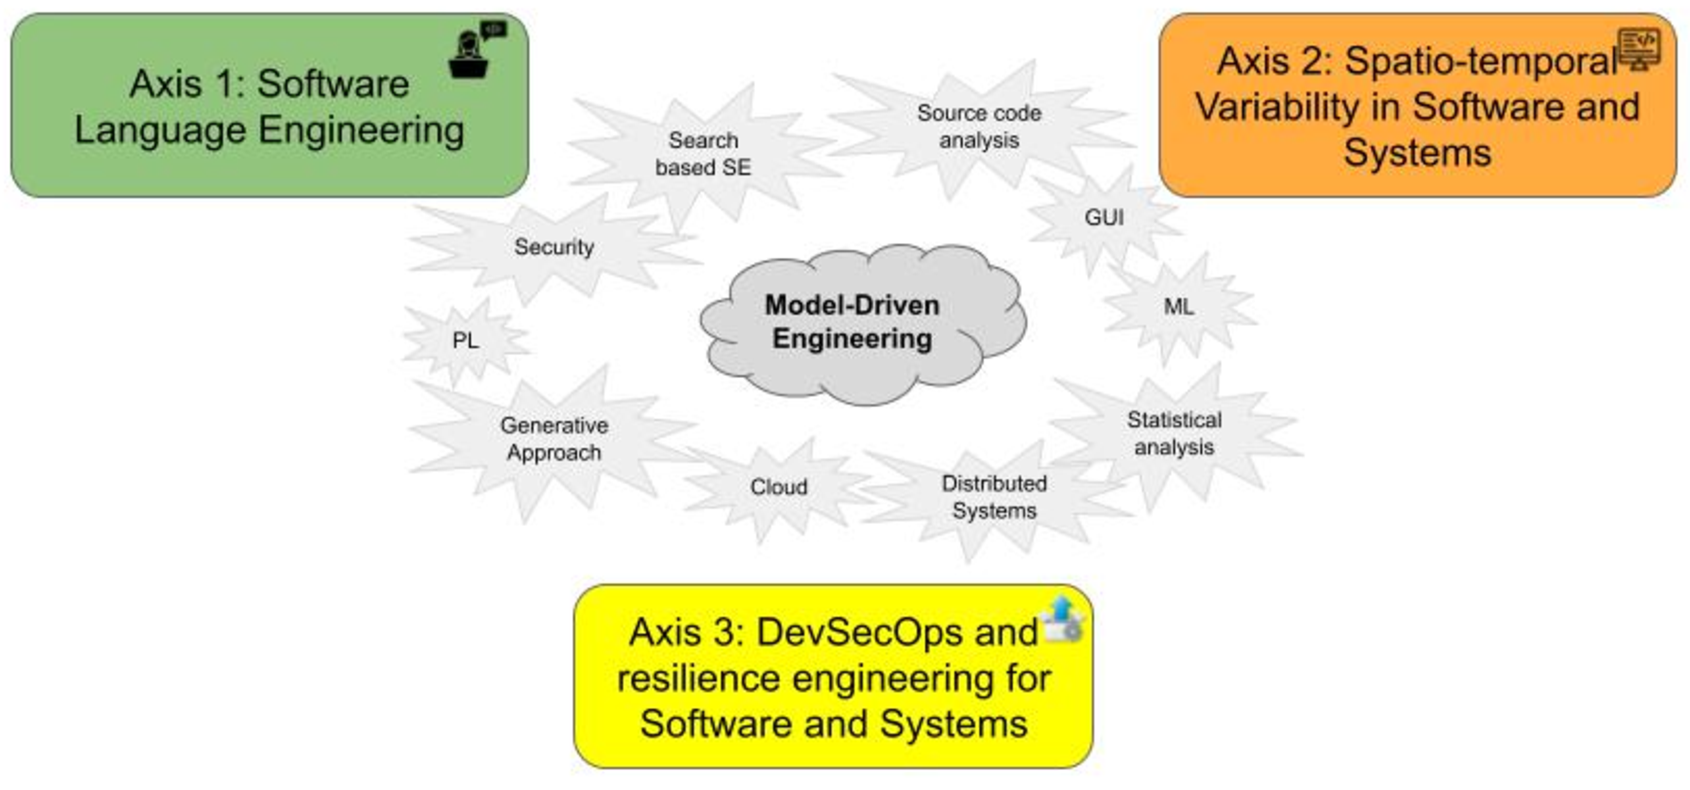
\includegraphics[width=0.7\columnwidth]{IMG/perspectives.pdf}
\caption{The three research axes of \team{}, relying on model driven engineering scientific background and leveraging several related fields}
\label{fig:perspectives}
\altdesc{The three research axes of \team{}, relying on model driven engineering scientific background and leveraging several related fields}
\end{figure}

%%%%%%%%%%%%%%
	
		\subsubsection{Axis \#1: Software Language Engineering} \label{sec:future-axis1-SLE}
		

\paragraph{Overall objective.} The disruptive design of new, complex systems requires a high degree of flexibility in the communication between many stakeholders, often limited by the silo-like structure of the organization itself (cf. Conway’s law). To overcome this constraint, modern engineering environments aim to: (i)~better manage the necessary exchanges between the different stakeholders; (ii)~provide a unique and usable place for information sharing; and (iii)~ensure the consistency of the many points of view. 
Software languages are the key pivot between the \emph{diverse} stakeholders involved, and the software systems they have to implement. 
Domain-Specific (Modeling) Languages enable stakeholders to address the \emph{diverse} concerns through specific points of view, and their coordinated use is essential to support the socio-technical coordination across the overall software system life cycle. 


Our perspectives on Software Language Engineering over the next period is presented in Figure~\ref{fig:perspectives-sle} and detailed in the following paragraphs.

\begin{figure}[h]
\centering
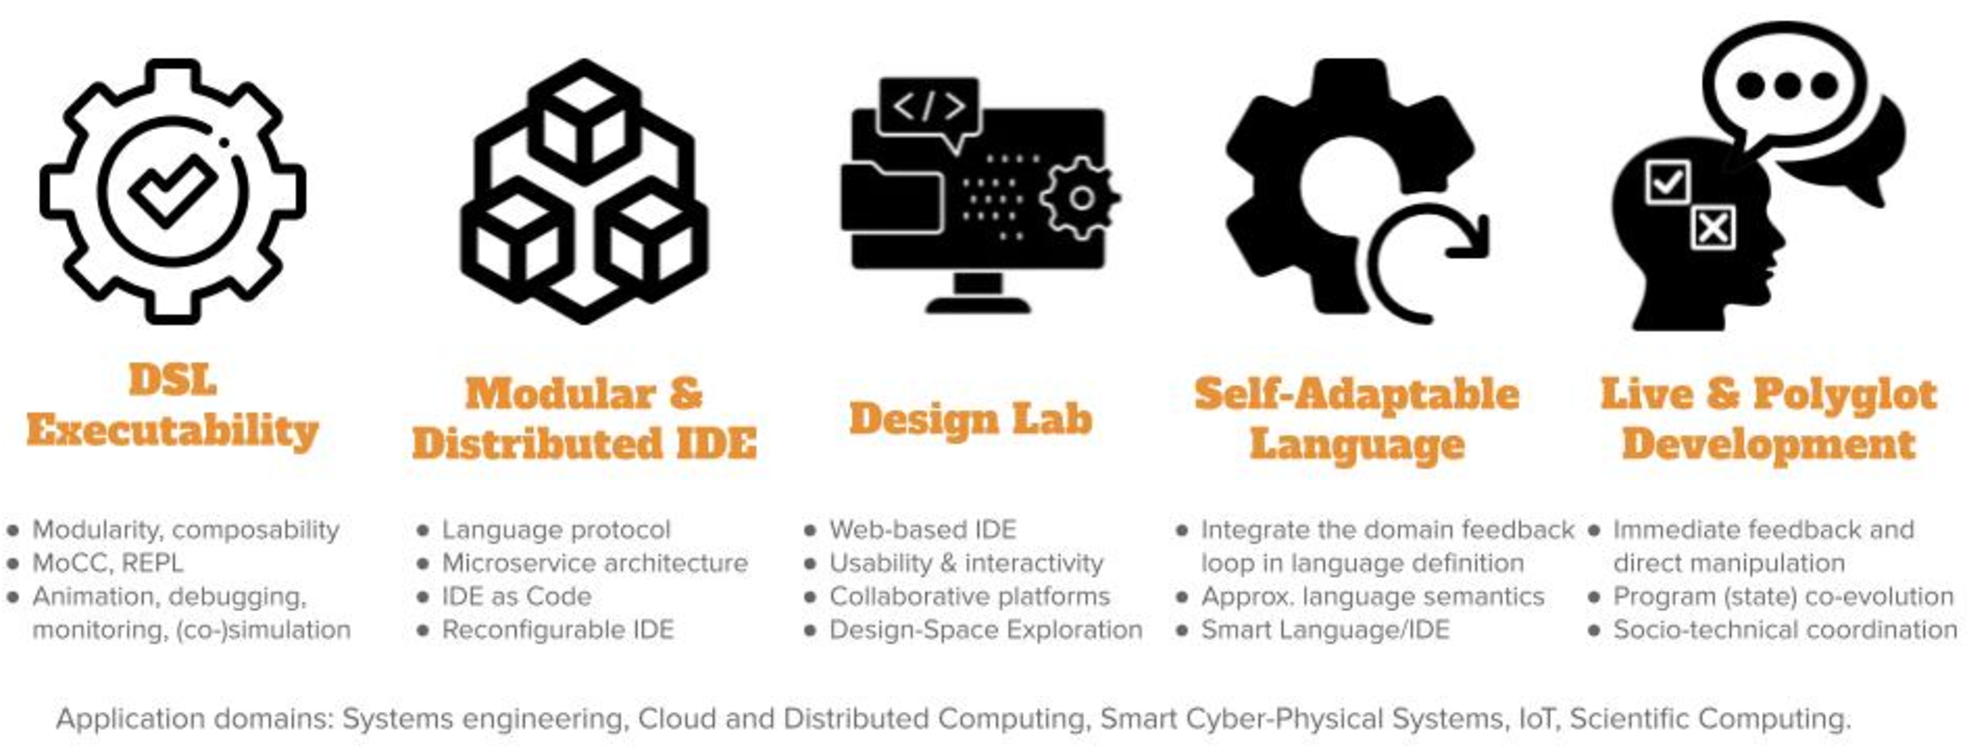
\includegraphics[width=\columnwidth]{IMG/sle.pdf}
\caption{Perspectives on Software Language Engineering (axis \#1)}
\label{fig:perspectives-sle}
\altdesc{Perspectives on Software Language Engineering (axis \#1)}
\end{figure}

\paragraph{DSL Executability.} Providing rich and adequate environments is key to the adoption of domain-specific languages. In particular, we focus on tools that support model and program execution. We explore the foundations to define the required concerns in language specification, and systematic approaches to derive environments (\emph{e.g.,} IDE, notebook, design labs) including debuggers, animators, simulators, loggers, monitors, trade-off analysis, etc.

\paragraph{Modular \& Distributed IDE.} IDEs are indispensable companions to software languages. They are increasingly turning towards Web-based platforms, heavily relying on cloud infrastructures and forges. Since all language services require different computing capacities and response times (to guarantee a user-friendly experience within the IDE) and use shared resources (\emph{e.g.,} the program), we explore new architectures for their modularization and systematic approaches for their individual deployment and dynamic adaptation within an IDE. To cope with the ever-growing number of programming languages, manufacturers of Integrated Development Environments (IDE) have recently defined protocols as a way to use and share multiple language services in language-agnostic environments. These protocols rely on a proper specification of the services that are commonly found in the tool support of general-purpose languages, and define a fixed set of capabilities to offer in the IDE. However, new languages regularly appear offering unique constructs (e.g., DSLs), and which are supported by dedicated services to be offered as new capabilities in IDEs. This trend leads to the multiplication of new protocols, hard to combine and possibly incompatible (e.g., overlap, different technological stacks). Beyond the proposition of specific protocols, we will explore an original approach to  be able to specify language protocols and to offer IDEs to be configured with such protocol specifications. IDEs went from directly supporting languages to protocols, and we envision the next step: \emph{IDE as code}, where language protocols are created or inferred on demand and serve as support of an adaptation loop taking in charge of the (re)configuration of the IDE. 

\paragraph{Design Lab.} Web-based and cloud-native IDEs open new opportunities to bridge the gap between the IDE and collaborative platforms, \emph{e.g.,} forges. In the complex world of software systems, we explore new approaches to reduce the distance between the various stakeholders (e.g., systems engineers and all those involved in specialty engineering) and to improve the interactions between them through an adapted tool chain. We aim to improve the usability of development cycles with efficiency, affordance and satisfaction. We also explore new approaches to explore and interact with the design space or other concerns such as human values or security, and provide facilities for trade-off analysis and decision making in the the context of software and system designs. 

\paragraph{Live \& Polyglot Development.} As of today, polyglot development is massively popular and virtually all software systems put multiple languages to use, which not only complexifies their development, but also their evolution and maintenance. Moreover, as software are more used in new application domains (e.g., data analytics, health or scientific computing), it is crucial to ease the participation of scientists, decision-makers, and more generally non-software experts. Live programming makes it possible to change a program while it is running, by propagating changes on a program code to its run-time state. This effectively bridges the gulf of evaluation between program writing and program execution: the effects a change has on the running system are immediately visible, and the developer can take immediate action. The challenges at the intersection of polyglot and live programming have received little attention so far, and we envision a language design and implementation approach to specify domain-specific languages and their coordination, and automatically provide interactive domain-specific environments for live and polyglot programming.

\paragraph{Self-Adaptable Language.} Over recent years, self-adaptation has become a concern for many software systems that operate in complex and changing environments. At the core of self-adaptation lies a feedback loop and its associated trade-off reasoning, to decide on the best course of action. However, existing software languages do not abstract the development and execution of such feedback loops for self-adaptable systems. Developers have to fall back to ad-hoc solutions to implement self-adaptable systems, often with wide-ranging design implications (e.g., explicit MAPE-K loop). Furthermore, existing software languages do not capitalize on monitored usage data of a language and its modeling environment. This hinders the continuous and automatic evolution of a software language based on feedback loops from the modeling environment and runtime software system. To address the aforementioned issues, we will explore the concept of Self-Adaptable Language (SAL) to abstract the feedback loops at both system and language levels.

	
		\subsubsection{Axis \#2: Spatio-temporal Variability in Software and Systems} \label{sec:future-axis2-variability}


 
\paragraph{Overall objective.} Leveraging our longstanding activity on variability management for software product lines and configurable systems covering \emph{diverse} scenarios of use, we will investigate over the next period the impact of such a variability across the \emph{diverse} layers, incl. source code, input/output data, compilation chain, operating systems and underlying execution platforms. We envision a better support and assistance for the configuration and optimisation (e.g., non-functional properties) of software systems according to this deep variability. Moreover, as software systems involve \emph{diverse} artefacts (\emph{e.g.,} APIs, tests, models, scripts, data, cloud services, documentation, deployment descriptors...), we will investigate their continuous co-evolution during the overall lifecycle, including maintenance and evolution. Our perspectives on spatio-temporal variability over the next period is presented in Figure~\ref{fig:perspectives-variability} and is detailed in the following paragraphs.

\begin{figure}[h]
\centering
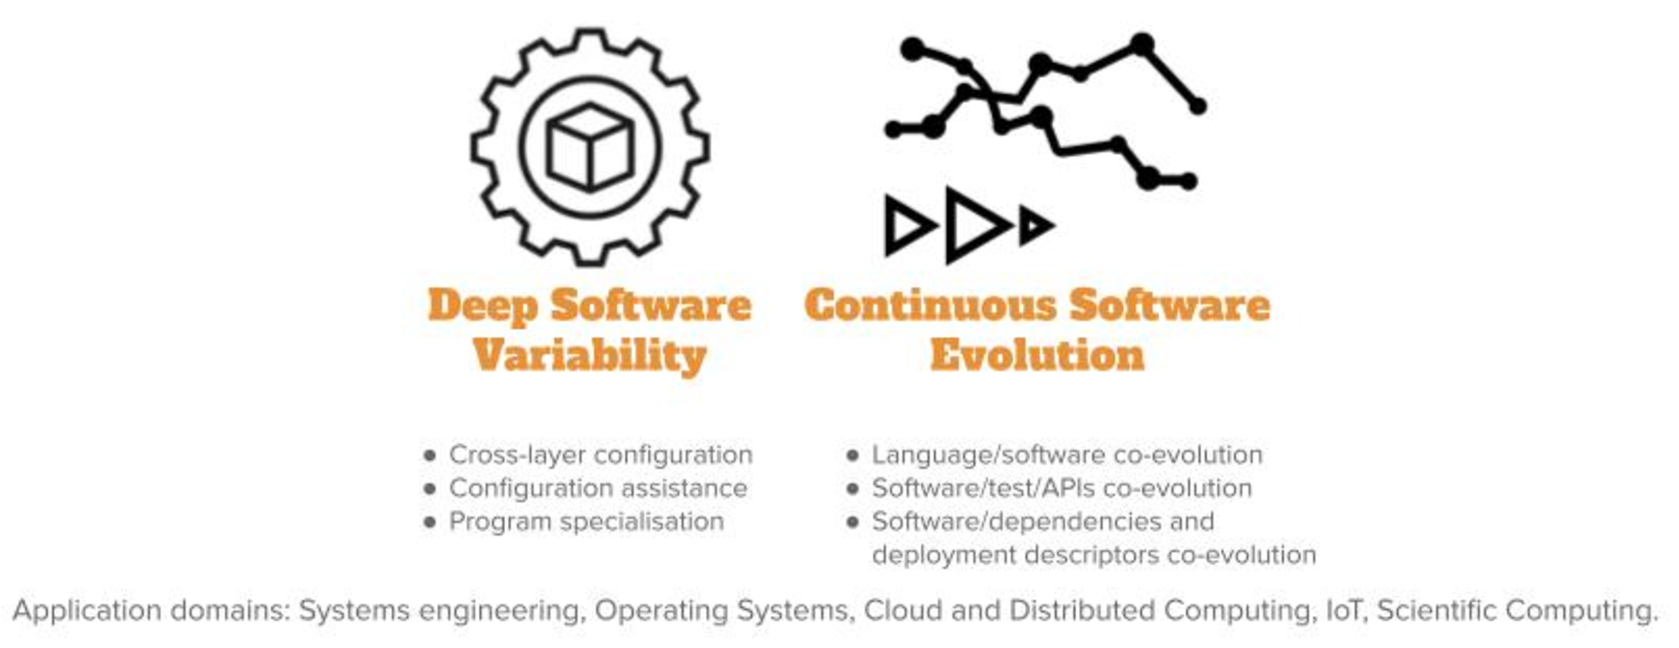
\includegraphics[width=\columnwidth]{IMG/variability.pdf}
\caption{Perspectives on Spatio-temporal Variability in Software and Systems (axis \#2)}
\label{fig:perspectives-variability}
\altdesc{Perspectives on Spatio-temporal Variability in Software and Systems (axis \#2)}
\end{figure}

\paragraph{Deep Software Variability.} Software systems can be configured to reach specific functional goals and non-functional performance, either statically at compile time or through the choice of command line options at runtime. We observed that considering the software layer only might be a naive approach to tune the performance of the system or to test its functional correctness.  In fact, many layers (hardware, operating system, input data, etc.), which are themselves subject to variability, can alter the performance or functionalities of software configurations. We call \emph{deep software variability} the interaction of all variability layers that could modify the behavior or non-functional properties of a software. Deep software variability calls to investigate how to systematically handle cross-layer configuration. The diversification of the different layers is also an opportunity to test the robustness and resilience of the software layer in multiple environments. Another interesting challenge is to tune the software for one specific executing environment. In essence, deep software variability questions the generalization of the configuration knowledge. 

\paragraph{Continuous Software Evolution.} Nowadays, software development has become more and more complex, involving various artefacts, such as APIs, tests, models, scripts, data, cloud services, documentation, etc., and embedding millions of lines of code (LOC). Recent evidence highlights continuous software evolution based on thousands of commits, hundreds of releases, all done by thousands of developers. We focus on the following essential backbone dimensions in software engineering: languages, models, APIs, tests and deployment descriptors, all revolving around software code implementation.  We will explore the foundations of a multidimensional and polyglot co-evolution platform, and will provide a better understanding with new empirical evidence and knowledge. 

	
		\subsubsection{Axis \#3: DevSecOps and Resilience Engineering for Software and Systems} \label{ sec:future-axis3-DevSecOps}

\paragraph{Overall objective.} The production and delivery of modern software systems involves the integration of \emph{diverse} dependencies and continuous deployment on \emph{diverse} execution platforms in the form of large distributed socio-technical systems. 
This leads to new software architectures and programming models, as well as complex supply chains for final delivery to system users. 
In order to boost cybersecurity, we want to provide strong support to software engineers and IT teams in the development and delivery of secure and resilient software systems, ie. systems able to resist or recover from cyberattacks.
Our perspectives on DevSecOps and Resilience Engineering over the next period are presented in Figure~\ref{fig:perspectives-devsecops} and detailed in the following paragraphs.


\begin{figure}[ht]
\centering
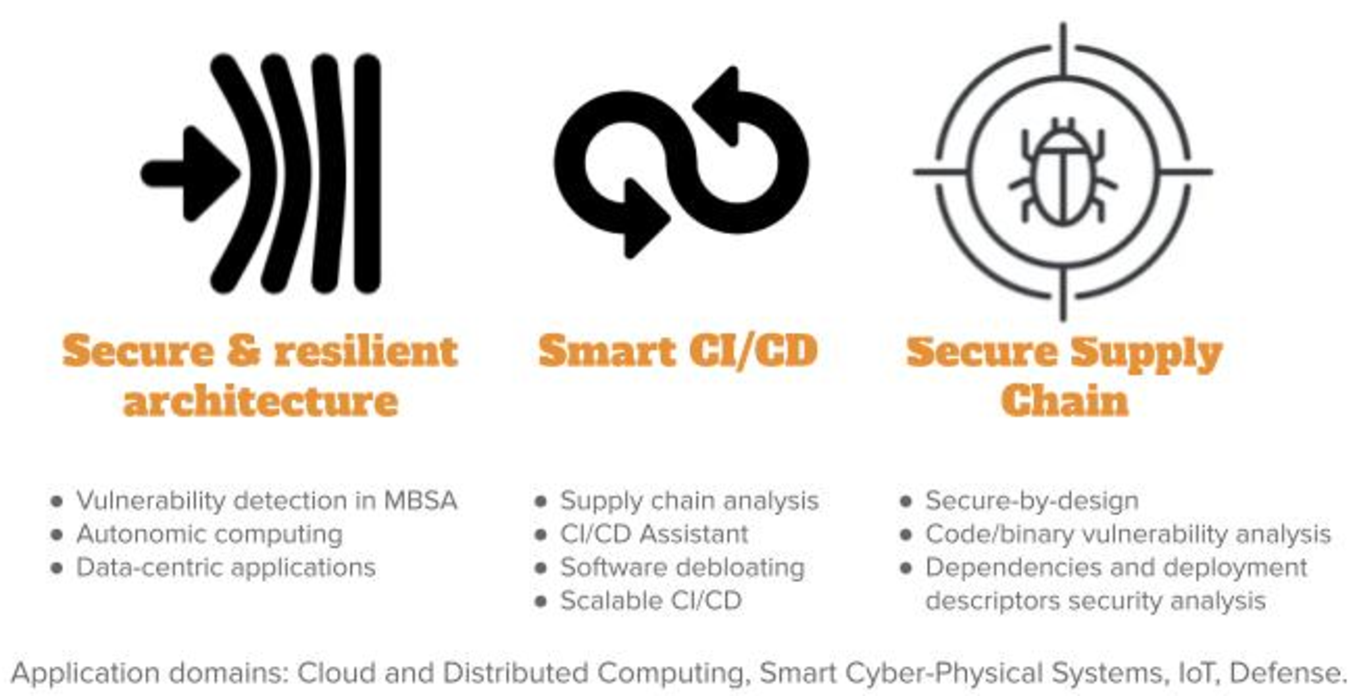
\includegraphics[width=.8\columnwidth]{IMG/devsecops.pdf}
\caption{Perspectives on DevSecOps and Resilience Eng. for Software and Systems (axis \#3)}
\label{fig:perspectives-devsecops}
\altdesc{Perspectives on DevSecOps and Resilience Eng. for Software and Systems (axis \#3)}
\end{figure}

\paragraph{Secure \& Resilient Architecture.} Continuous integration and deployment pipelines are processes implementing complex software supply chains. We envision an explicit and early consideration of security properties in such pipelines to help in detecting vulnerabilities. In particular, we integrate the security concern in Model-Based System Analysis (MBSA) approaches, and explore guidelines, tools and methods to drive the definition of secure and resilient architectures. We also investigate resilience at runtime through frameworks for autonomic computing and data-centric applications, both for the software systems and the associated deployment descriptors. 

\paragraph{Smart CI/CD.} Dependencies management, Infrastructure as Code (IaC) and DevOps practices open opportunities to analyze complex supply chains. We aim at providing relevant metrics to evaluate and ensure the security of such supply chains, advanced assistants to help in specifying corresponding pipelines, and new approaches to optimize them (\emph{e.g.,} software debloating, scalability\ldots).
We study how supply chains can actively leverage software variability and diversity to increase cybersecurity and resilience. 

\paragraph{Secure Supply Chain.} In order to produce secure and resilient software systems, we explore new secure-by-design foundations that integrate security concerns as first class entities through a seamless continuum from the design to the continuous integration and deployment. 
We explore new models, architectures, inter-relations, and static and dynamic analyses that rely on explicitly expressed security concerns to ensure a secure and resilient supply chain. 
We lead research on automatic vulnerability and malware detection in modern supply chains, considering the various artefacts either as white boxes enabling source code analysis (to avoid accidental vulnerabilities or intentional ones or code poisoning), or as black boxes requiring binary analysis (to find malware or vulnerabilities).
We also conduct research activities in dependencies and deployment descriptors security analysis. 


%% [END last year imported content]
